\section{Analiza sistema}
\label{sec:naslov1}
 
Informacioni sistem je namenjen kandidatima tj. ljudima koji žele da završe vozačku obuku, kao i zaposlenima u toj auto školi. 
Sistem prikazuje način funkcionisanja jedne konkretne auto škole, a može se iskoristiti za unapređenje načina rada postojećih sistema u okviru auto škola.
U nastavku su opisani akteri koje smo prepoznali, kao i njihove uloge u ovom sistemu.

\
\subsection {Akteri}
\label{subsec:podnaslov1}
\begin{itemize}
\item \textbf{Administrator sistema} – Nalazi se na vrhu hijerarhije zaposlenih. Zadužen je direktno ili indirektno za većinu procesa u auto školi. Njegova uloga je takođe da održava bazu podataka. On vrši ažuriranje baze, dodavanjem novog klijenta kada dobije informacije od administrativnog radnika i šalje mejl potvrde kandidatu da je registrovan sa njegovim ID-jem i lozinkom.
\item \textbf{Administrativni radnik} – Na osnovu obrade podataka za prijavljenog kandidata formira kompletnu administrativnu dokumentaciju koja prati kandidata od upisa do izdavanja vozačke dozvole. Šalje podatke o kandidatu administratoru i kroz to zahteva njegovu registraciju u bazi podataka. Komunicira sa kandidatom i održava te podatke. Formira zapisnik teorijske i praktične provere.
\item \textbf{Računovođa} – Zadužen je za finansije. Vodi evidenciju o svim uplatama kandidata, o isplati plata zaposlenima i o održavanju cenovnika usluga.
\item \textbf{Nadležni za zapsolene} – Formira evidenciju kadrova(instruktora, predavača, računovođa, administrativnih radnika) i vodi računa o rasporedu rada. Vodi evidenciju o vozilima i opremi u auto školi.
\item \textbf{Predavači} – Održavaju časove, pripremaju materijale i kratke provere znanja. Imaju uvid o grupama i broju kandidata u svakoj grupi. Vode evidenciju o prisutnima na času predavanja.
\item \textbf{Instruktori} – Drže časove vožnje i vrše zakazivanje časova u dogovoru sa kandidatima. Upisuju u sistem podatke o održanom času. Imaju evidenciju o kandidatima koji su im dodeljeni. Vrše zapisnik o polaganju vozačkog ispita na kome su prisutni.
\item \textbf{Kandidati} – Prijavljuje se za obuku u auto školi  popunjavanjem online forme, unoseći svoje lične podatke i prilažući potrvdu o izvršenoj uplati. Na mejl dobija potvrdu da je registrovan i podatke za prijavu(ID i šifru). Na svom profilu može videti sve neophodne informacije, kao i proveriti ispravnost svojih podataka. Potrebno je da izvrši izbor grupe za teorijsku obuku. Nakon položene teorijske obuke, neophodno je da izabere instruktora i onda započinje praktičnu obuku. Časove zakazuje u dogovoru sa instruktorom, a neophodno je da se realizuje 40 časova praktične obuke(vožnje). Nakon toga, prijavljuje se za izlazak na vozački ispit odabirom željenog termina na formi. Ukoliko uspešno položi vozački ispit, neophodno je da popuni anketu o auto školi i dobija potvrdu o obavljenoj obuci u auto školi. U suprotnom, bira termin za novi izlazak na vozački ispit. 
\end{itemize}

Na slici  \label{fig:kontekst} su predstavljeni svi akteri sistema kroz dijagram konteksta.
\begin{figure}[H]
    \begin{center}
        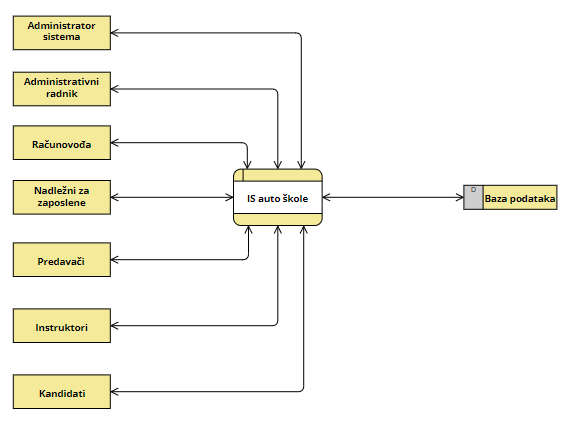
\includegraphics[width=120mm, height=60mm]{Diagrams/dijagram_konteksta.png}
    \end{center}
    \caption {Dijagram konteksta}
    \label{fig:kontekst}

\end{figure}